\documentclass[10pt]{article}
\usepackage{icmlko}

\icmlmeta{IP 파운데이션 월드모델}{244}{적게 보면 더 잘 보인다}{안쪽이 작은 변화를 못 읽는 것은 조각이 적어서가 아니라 옛 시대를 섞어서다}

\begin{document}

\twocolumn[
\icmlheader

\begin{abstract}
노트 243은 안쪽 눈금이 $|\Delta| \le 0.010$ 에서 동전 던지기임을 쟀다
(spearman $+$0.36). 왜인지 갈랐다. \textbf{예측을 먼저 적고 쟀다} --- 조각이
셋뿐이라 분산이 크니 여섯으로 늘리면 나아질 것이다. \textbf{틀렸다}: 반해
여섯이 $+$0.21, 해 다섯이 $+$0.20 으로 셋($+$0.36)보다 \emph{나쁘다}. 두 번째
가설은 ``그 크기가 아예 측정 바닥 아래''였다. 유보를 무작위로 반 갈라 같은
변화를 두 번 재니 \textbf{반쪽끼리 spearman $+$0.63 · 부호 11/13} 이다
(스피어만--브라운으로 온전한 유보의 신뢰도 $\approx$0.78). \textbf{유보는 그
칸을 읽는다.} 남은 답은 하나였다 --- 조각을 \emph{줄이고} 경계에 붙이면
어떻게 되나. 2024 한 조각(평가 1,121건)이 $+$0.51 로 해 셋(3,245건)의
$+$0.36 을 이긴다. \textbf{자료를 3분의 1만 쓰는데 더 잘 읽는다.} 안쪽의
약점은 분산이 아니라 \textbf{시대 섞기}였다 --- 2022 · 2023 조각은 2025를
닮지 않았고, 평균을 내면 그 편향이 신호를 덮는다. 노트 200이 ``접힘 교차는
시간을 섞어 부호를 반대로 본다''고 적은 것과 같은 병이 한 층 위에서 났다.
신뢰도로 환산하면 안쪽은 해 셋에서 $\le$0.16, 한 조각에서 $\le$0.34 다
(유보 0.78 대비). \texttt{tune.inner\_split} 은 \textbf{이미} 앞으로 한 번만
가르고 있었다 --- 실험실은 맞게 하고 있었고, 틀린 것은 내가 노트 241 · 243
에서 근거로 쓴 \emph{세 조각 평균}이다.
\end{abstract}
]

\section{예측을 적고 쟀다}

노트 243이 남긴 표의 첫 줄은 ``안쪽 조각을 셋에서 다섯 · 여섯으로 늘리면
작은 칸이 보이나''였다. 늘리면 나아질 것이라는 예측에는 이유가 있다 ---
조각마다 평가 표본이 1,000건 남짓이니 평균이 흔들릴 것이고, 조각을 늘리면
그 흔들림이 준다.

\textbf{예측을 먼저 적어 두고} 쟀다. 노트 243이 만든 열일곱 점(축 하나씩
빼기)의 유보 값은 그대로 두고 안쪽만 다시 계산했다.

\begin{center}\small
\begin{tabular}{lrrr}
\hline
안쪽 방식 & 조각 & 전체 & 작은 칸 \\
\hline
해 셋 (지금) & 3 & $+$0.691 & $+$0.357 \\
해 다섯 & 5 & $+$0.627 & $+$0.203 \\
반해 여섯 & 6 & $+$0.632 & $+$0.214 \\
\hline
\end{tabular}
\end{center}

늘리니 \emph{나빠졌다}. 예측이 반증됐다.

\section{바닥이 아니다}

두 번째 가설 --- $|\Delta| \le 0.010$ 은 유보 2,565건으로도 못 재는 크기라
안쪽이 아니라 \emph{양쪽이} 잡음이다. 이게 맞다면 실험실이 다투는 변화의
대부분이 잡음이라는 뜻이라, 먼저 확인해야 했다.

유보를 도메인마다 무작위로 반 갈라, 같은 열일곱 변화를 두 반쪽에서 따로
쟀다.

\begin{figure}[t]
\centering
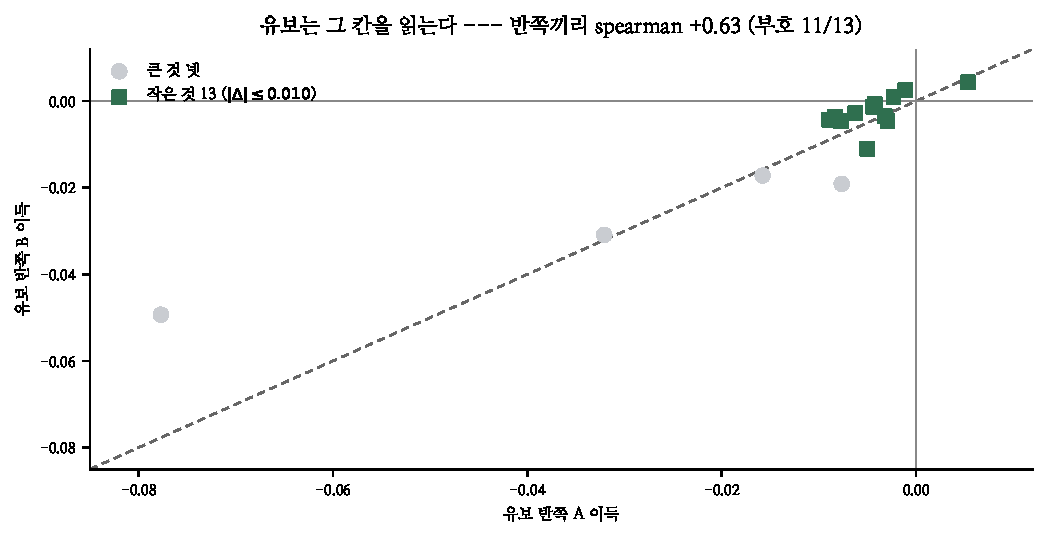
\includegraphics[width=\columnwidth]{figs/halves.pdf}
\caption{유보 반쪽 A 대 반쪽 B. 초록 열셋이 작은 칸인데, 반쪽끼리도
같은 방향으로 움직인다.}
\end{figure}

\begin{center}\small
\begin{tabular}{lrr}
\hline
 & spearman & 부호 \\
\hline
열일곱 전부 & $+$0.781 & 15/17 \\
작은 것 열셋 & $+$0.633 & 11/13 \\
\hline
\end{tabular}
\end{center}

반쪽(1,283건)끼리 $+$0.633 이면 스피어만--브라운으로 온전한 유보의 신뢰도는
$2r/(1+r) \approx 0.78$ 이다. \textbf{유보는 그 칸을 잘 읽는다.} 바닥이
아니었다.

\section{줄이고 경계에 붙였다}

늘려서 나빠졌으니 줄여 봤다. 그리고 어디에 두느냐를 같이 봤다 --- 실제
과제는 ``2025 이전 전부로 배워 2025 이후를 맞힌다''이므로, 그것을 제일
닮은 안쪽은 \textbf{경계 바로 앞 한 조각}이다.

\begin{figure}[t]
\centering
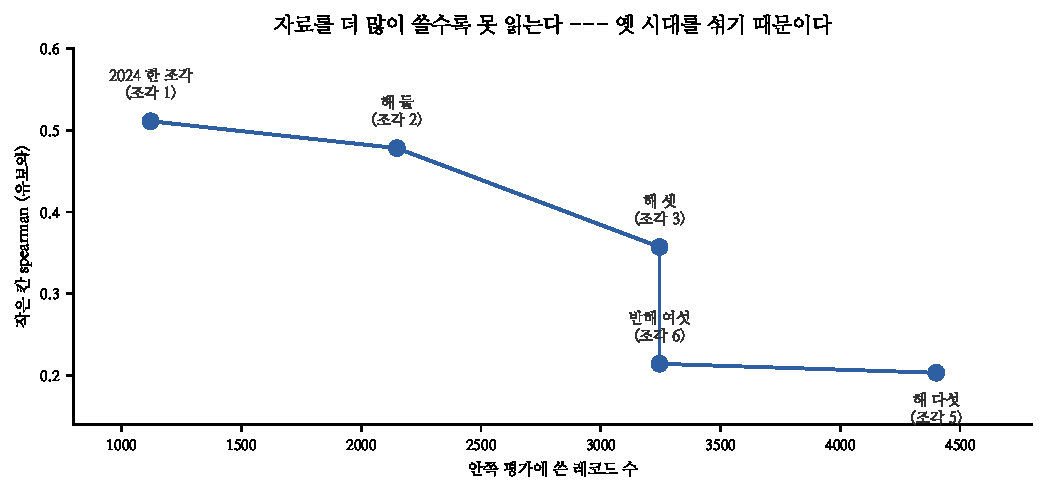
\includegraphics[width=\columnwidth]{figs/slices.pdf}
\caption{안쪽 평가에 쓴 레코드 수와 작은 칸 읽기. 자료를 많이 쓸수록
못 읽는다.}
\end{figure}

\begin{center}\small
\begin{tabular}{lrrr}
\hline
안쪽 방식 & 평가 건수 & 전체 & 작은 칸 \\
\hline
해 셋 & 3,245 & $+$0.691 & $+$0.357 \\
해 둘 (2023 · 2024) & 2,149 & $+$0.760 & $+$0.478 \\
\textbf{2024 한 조각} & \textbf{1,121} & $\mathbf{+0.775}$ & $\mathbf{+0.511}$ \\
\hline
\end{tabular}
\end{center}

\textbf{자료를 3분의 1만 쓰는데 더 잘 읽는다.} 분산 이야기였다면 있을 수
없는 방향이다. 남는 설명은 \textbf{편향}이다 --- 2022 · 2023 조각은 2025를
닮지 않았고, 그것을 평균에 넣으면 답이 아니라 \emph{다른 질문의 답}이
섞인다.

이 실험실은 이 병을 이미 한 번 앓았다. 노트 200이 ``접힘 교차는 시간을 섞어
부호를 반대로 본다''고 적고 도메인별 풀링 격차를 \emph{앞으로 두 토막}으로
재도록 고쳤다. 같은 병이 한 층 위, \textbf{조각을 평균하는 자리}에서 다시
났다.

\section{신뢰도로 환산하면}

관측 상관은 $r_{\text{obs}} = \sqrt{\rho_i \rho_h}\, r_{\text{true}}$ 이다.
$\rho_h = 0.78$ 이고 $r_{\text{true}} \le 1$ 이니 안쪽 신뢰도의 \emph{상한}이
나온다.

\begin{center}\small
\begin{tabular}{lrr}
\hline
안쪽 방식 & 작은 칸 $r$ & 신뢰도 상한 \\
\hline
해 셋 & $+$0.357 & $\le$ 0.16 \\
2024 한 조각 & $+$0.511 & $\le$ 0.34 \\
유보(온전) & --- & 0.78 \\
\hline
\end{tabular}
\end{center}

한 조각으로 바꿔도 유보의 절반에 못 미친다. \textbf{작은 칸에서 안쪽은
여전히 약하다} --- 다만 쓸모없지는 않다.

\section{실험실은 맞게 하고 있었다}

고칠 곳을 찾아 \texttt{lab/tune.py} 를 열었더니 \texttt{inner\_split} 은
\textbf{이미} 학습 구간을 시간으로 한 번만(7 대 3) 가르고 있었다. 조각을
평균하는 곳은 \texttt{tune.stable} 의 다섯 자리뿐인데, 그 다섯을 최근 쪽
(0.70$\sim$0.90)으로 옮겨도 판이 넷째 자리까지 안 움직인다 --- 지금 판에서
$\tau$ 가 어차피 꺼져 있기 때문이다(노트 243).

\textbf{그러니 고칠 것은 코드가 아니라 나다.} 노트 241과 243에서 내가 근거로
쓴 안쪽 숫자는 손으로 짠 \emph{세 조각 평균}이었고, 그게 제일 나쁜 방식이었다.
노트 241의 결론(도메인별 기울기 거부)은 그대로다 --- 한 조각으로 다시 재도
그 쌍들은 여전히 작은 칸에 있고, 안쪽 신뢰도 상한이 0.34 라 근거가 못 된다.

\paragraph{남은 것}
\begin{center}\small
\begin{tabular}{ll}
\hline
갈래 & 왜 \\
\hline
왜 2022가 다른가 & 시대 편향의 정체. 라벨 누적(노트 209)인가 \\
안쪽 0.34 & 더 올릴 길이 있나. 아니면 작은 칸을 포기하나 \\
\texttt{entry\_friction} & 빼면 $-$0.0637 --- 판에서 제일 무거운 손 축 \\
\texttt{venue\_prominence} & 안쪽 $-$0.0010 인데 유보 $-$0.0089 \\
\hline
\end{tabular}
\end{center}

\paragraph{규약} 안쪽 숫자를 근거로 쓸 때는 \textbf{경계 바로 앞 한 조각}에서
잰다. 조각을 여럿 평균하지 않는다 --- 옛 조각은 표본을 더 주는 게 아니라
다른 시대를 섞는다.

\end{document}
